\documentclass[a4paper,11pt,french]{article}
\usepackage[utf8]{inputenc}

\usepackage[T1]{fontenc}
\usepackage[francais]{babel} 
\usepackage[top=2cm, bottom=2cm, left=2cm, right=2cm, includeheadfoot]{geometry} %pour les marges
\usepackage{lmodern}
\usepackage{pict2e}
\usepackage{tikz}	
\usepackage{tikz-uml}
\usepackage{fancyhdr}   % Required for custom headers
\usepackage{lastpage}   % Required to determine the last page for the footer
\usepackage{extramarks} % Required for headers and footers
\usepackage{graphicx}   % Required to insert images
\usepackage{tabularx, longtable}
\usepackage{color, colortbl}
\usepackage[toc,page]{appendix} 
\usepackage{pgfplots}
\usepackage{eurosym}
\usepackage{rotating}
\usepackage{array}

\geometry{a4paper,textwidth=17cm,textheight=27cm} 

\usetikzlibrary{trees,shapes.geometric,arrows,decorations.pathmorphing,backgrounds,fit,positioning,shapes.symbols,chains	}
 \tikzset{
    %Define standard arrow tip
    >=stealth',
    %Define style for boxes
    punkt/.style={
           rectangle, dashed,
           rounded corners,
           draw=black, very thin,
           minimum height=2em,
           minimum width = 2cm,
           text centered},
    square/.style={
           rectangle,
           draw=black, thick,
           minimum height=.5cm,
           minimum width = 1cm,
           text centered},
    data/.style={
           rectangle,
           draw=black, thick,
           minimum height= 2cm,
           minimum width = 2cm,
           text centered},
    % Define arrow style
    pil/.style={
           ->,
           thick,
           shorten <=1pt,
           shorten >=1pt,},
    asym/.style={
           <->,
           thin,
           shorten <=1pt,
           shorten >=1pt,
           red!100},
    sym/.style={
           <->,
           thin,
           shorten <=1pt,
           shorten >=1pt,
           blue!100}
}

\usepgflibrary{arrows} % for pgf-umlsd

\linespread{1.1} % Line spacing

% Set up the header and footer
\pagestyle{fancy}
\lhead{\textbf{\hmwkClass -- \hmwkSubject \\ \hmwkTitle \\ \hmwkDocName}} % Top left header
\rhead{
\includegraphics[width=10em]{logo_univ.png}}
\lfoot{\lastxmark} % Bottom left footer
\cfoot{} % Bottom center footer
\rfoot{Page\ \thepage\ / \pageref{LastPage}} % Bottom right footer
\renewcommand\headrulewidth{0.4pt} % Size of the header rule
\renewcommand\footrulewidth{0.4pt} % Size of the footer rule

\setlength{\headheight}{40pt}

\newcommand{\hmwkTitle}{Chat sécurisé} % Assignment title
\newcommand{\hmwkClass}{Master 1 SSI } % Course/class
\newcommand{\hmwkClassInstructor}{Jones} % Teacher/lecturer
\newcommand{\hmwkAuthorName}{Yves Nouafo} % Your name
\newcommand{\hmwkSubject}{Conduite de projet} % Subject
\newcommand{\hmwkDocName}{Architecture du logiciel} % Document name

\newcommand{\version}{1.1} % Document version
\newcommand{\docDate}{24 mai 2013} % Document date
\newcommand{\checked}{Julien Legras} % Checker name
\newcommand{\approved}{Magali Bardet} % Approver name

\newcommand{\fiche}[9] {
	\noindent
\begin{tabular}{|p{3.5cm}| p{1cm} | p{3cm} | p{.5cm} | p{7cm}|} 
\hline
\rowcolor{blue}
\multicolumn{2}{|l|}{\color{white}\bfseries{Nom}} & \multicolumn{3}{l|}{\color{white}\bfseries{#1}}\\
\hline
\multicolumn{2}{|l|}{\bfseries{Acteurs concernés}} & \multicolumn{3}{m{10.5cm}|}{#2}\\
\hline
\multicolumn{2}{|l|}{\bfseries{Description}} & \multicolumn{3}{m{10.5cm}|}{#3}\\
\hline
\multicolumn{2}{|l|}{\bfseries{Préconditions}} & \multicolumn{3}{m{10.5cm}|}{#4}\\
\hline
\multicolumn{2}{|l|}{\bfseries{Evénements déclenchants}} & \multicolumn{3}{m{10.5cm}|}{#5}\\
\hline
\multicolumn{2}{|l|}{\bfseries{Conditions d'arrêt}} & \multicolumn{3}{m{10.5cm}|}{#6}\\
\hline
\rowcolor{gray}
\multicolumn{5}{|c|}{\bfseries{Description du flot d'événements principal}}\\
\hline
\rowcolor{gray}
\multicolumn{3}{|c|}{\bfseries{Acteur(s)}} & \multicolumn{2}{c|}{\bfseries{Système}}\\
\hline
\multicolumn{3}{|p{7.5cm}|}{#7} & \multicolumn{2}{p{7.5cm}|}{#8}\\
\hline
\multicolumn{2}{|l}{\bfseries{Flots d'exceptions}} & \multicolumn{3}{|p{11.5cm}|}{#9}\\
\hline
\end{tabular}
\\
}

\definecolor{gris}{rgb}{0.95, 0.95, 0.95}

\author{\hmwkAuthorName}
\date{} % Insert date here if you want it to appear below your name


\begin{document}
\pagestyle{fancy}

\vspace*{5cm}
\begin{center}\textbf{\Huge{\hmwkDocName}}\end{center}
\vspace*{4cm}
	
\fcolorbox{black}{gris}{
\begin{minipage}{15cm}
\begin{tabularx}{10cm}{lXl}
	\bfseries{Version} & & \version\\
	& & \\
	\bfseries{Date} & & \docDate\\
	& & \\
	\bfseries{Rédigé par} & & \hmwkAuthorName \\
	& & \\
	\bfseries{Relu par} & & \checked \\
	& & \\
	\bfseries{Approuvé par} & & \approved \\
	& & \\
\end{tabularx}
\end{minipage}
}

\newpage

%Tableau de mises à jour
\vspace*{1cm}
\begin{center}
\vspace*{2cm}
\textbf{\huge{MISES À JOUR}}\\
\vspace*{4cm}
	\begin{tabularx}{16cm}{|c|c|X|}
	\hline
	\bfseries{Version} & \bfseries{Date} & \bfseries{Modifications réalisées}\\
	\hline
	0.1 & 16/11/2012 & Création\\
	\hline
	0.2 & 23/11/2012 & Avancement des schémas et complétion du document\\
	\hline
	0.3 & 1/12/2012 & Modificatoin des schémas UML\\
	\hline
	0.4 & 12/12/2012 & Ajout UC.19 – UC.18 – UC.17\\
	\hline
	0.5 & 14/12/2012 & Modification après réunion du 12/12/12\\
	\hline
	0.6 & 30/12/2012 & Ajout du schéma globale de l'application et de la partie sur la cryptographie\\
	\hline
	1.1 & 24/05/2013 & Mise à jour du document conformément aux modifications apporté\\
	\hline
	\end{tabularx}
\end{center}

%La table des matières
\clearpage
\tableofcontents
\clearpage
%--------------------------------------------------
\section{Objet}
Le présent document montre l'architecture utilisée pour réaliser un système de bavarde (ou chat en anglais) sécurisé. Plusieurs modules seront développés de manière indépendante, chacune ayant un rôle bien définie. Les différentes entités pourront communiquer entre elles et devront respecter les critères suivant:\\
\begin{itemize}
\item Gestion de la création et de la suppression d’un compte sécurisé;
\item Création par un utilisateur d’une salle de discussion pour un groupe de personnes;
\item Ajout/suppression d’un utilisateur autorisé dans une salle privé;
\item Confidentialité, intégrité et authentification sur les messages échangés;
\item Non-répudiation possible des messages;
\item Création d’une autorité de certification;
\item Demande de certificat pour accès au salon privé et communication sécurisé;
\end{itemize}

%-------------------------------------------------
\section{Documents applicables et de référence}
\begin{itemize}
\item IRC (RFC 2810 à 2813 de avril 2000)
\item STB (Spécification Technique des Besoins)
\end{itemize}

%-------------------------------------------------
\section{Terminologie et sigles utilisés}
\begin{itemize}
\item \textbf{Public Key Infrastructure (PKI)} : Infrastructure de gestion des clés publiques qui permet de gérer clés publiques et d'en assurer la fiabilité pour des entités dans un réseaux. Elle permet un échange sécurisé des informations en garantissant les principaux points de la cryptographie: l'intégrité, l'authentification, la confidentialité et la non-répudiation lors d'échanges d'informations.
%\item \textbf{Autorité de certification (AC)} : Organisme qui à pour mission de signer les demandes de certificat et de signer les listes de révocation.
\item \textbf{Autorité d'enregistrement (AR)} : Organisme qui génère les certificats et effectue les vérifications d'usage sur les utilisateurs.
\item \textbf{Confidentialité} : Les informations échangées deviennent illisibles, cette confidentialité est assurée par le chiffrement.
\item \textbf{Non-répudiation} : L'émetteur des données ne peut pas nier être à l'origine du message.
\item \textbf{Intégration} : Fonctionnement permettant d'assurer que l'information n'a pas subi de modification.
\item \textbf{Signature} : Code électronique unique qui permet de signer un message codé. Elle permet d'identifier l'origine du message.
\item \textbf{Certificat} : Document électronique qui fait correspondre une clé avec une entité. Cette correspondance est validée par une autorité de certification.
\item \textbf{Authentification (Authent)} : connexion sur le chat via un identifiant.
\item \textbf{Authentification sécurisé (Authent S)} : Identification de l'origine de l'information.
\item \textbf{Liste de dépots (LDD)} :  A pour mission de stocker les certificats numériques ainsi que les listes de révocation. 
\item \textbf{Client sécurisé (Client S)} :  A pour mission de chiffrer et déchiffrer les messages.
\item \textbf{Base de données (BDD)} : Conteneur informatique permettant de stocker dans un même endroit l'intégralité des informations.

\end{itemize}

%-------------------------------------------------
\section{Configuration requise}
\vspace{0.8cm}
\subsection{Performances du calculateur}
\begin{itemize}
\item 1Go RAM 
\item Intel Celeron
\item Virtual Machine (VM)
\end{itemize}
\vspace{0.3cm}
\subsection{Système d’exploitation}
\begin{itemize}
\item Ubuntu 12.04 LTS
\end{itemize}
\vspace{0.3cm}
\subsection{Produits logiciels nécessaires}
\begin{itemize}
\item EJBCA pour la mise en place de la PKI et la délivrance des certificats
\item OpenSSL pour l'apport de la bibliothèque cryptographique
\item GTK 3
\end{itemize}
%-------------------------------------------------

\vspace{0.8cm}
\section{Architecture statique}
\vspace{0.3cm}
\subsection{Structure}
Les principales parties à développer:
\begin{itemize}
\item L'application client: le système de bavardage
\item Les serveurs:
\begin{itemize}
\item Le serveur non sécurisé
\item Le serveur sécurisé
\item La PKI avec: AC, AR, politique de certification
\end{itemize}
\item Les données:
\begin{itemize}
\item Liste de dépots (LDD)
\item Bases de données non persistante (liste chainée) gérant les utilisateurs non sécurisés
\item Bases de données persistante gérant les utilisateurs sécurisés
\end{itemize}
\end{itemize}

%\begin{figure}[!htbp]
%\centerline{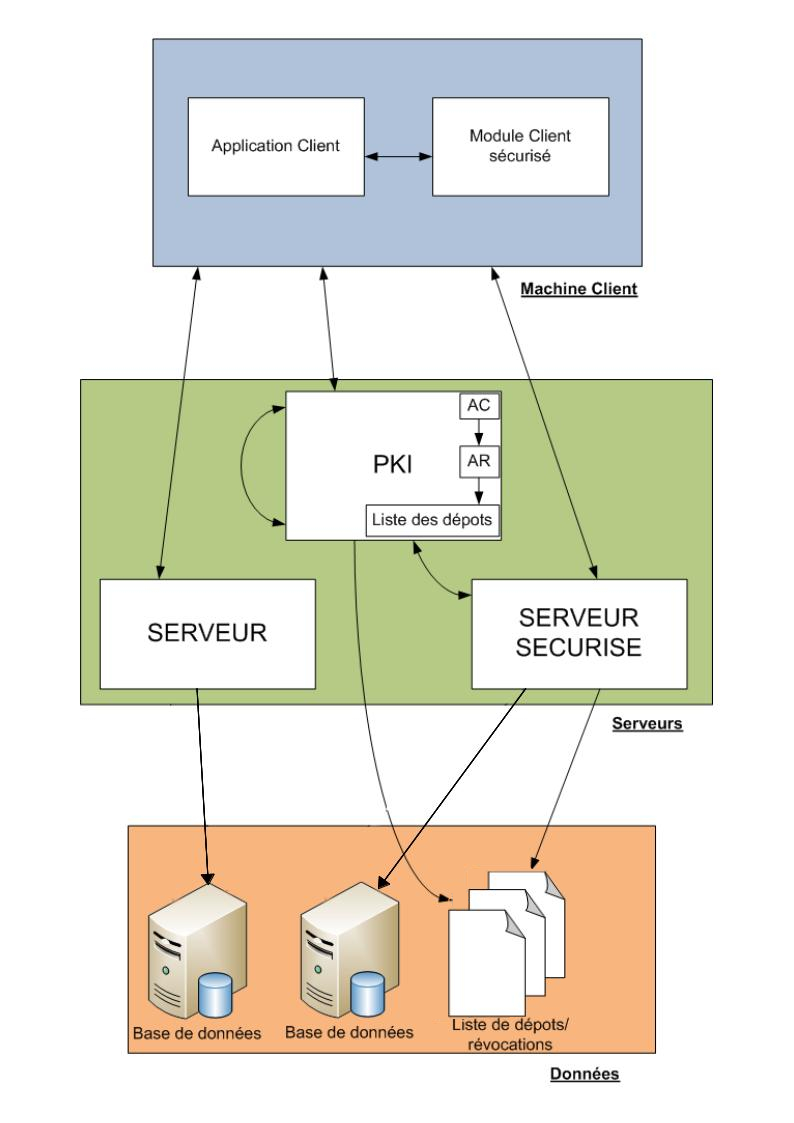
\includegraphics[width=12cm]{Arch.jpg} }
%\caption{Fonctionnement de l'application}
%\end{figure}
\vspace{4cm}
\begin{tikzpicture}[node distance=-.01cm,font=\tiny,scale=3.0,every node/.style={transform shape}]
		\node[square, text width=1cm, fill=white!100] (appclient) at (0,0) {Application client};
		\node[square, text width=1.5cm, fill=white!100] (modclientsec) at (2.5,0) {Module client sécurisé};
		\begin{pgfonlayer}{background} 
		\node[punkt, fit=(appclient)(modclientsec), fill=blue!20] (groupclient) {};
		\end{pgfonlayer}
		
		\node[square, text width=1cm, fill=white!100] (PKI) at (1.4,-1.5) {PKI};
		\node[square, text width=1cm, fill=white!100] (serveur) at (0,-2.5) {Serveur};
		\node[square, text width=1.5cm, fill=white!100] (serveurs) at (2.5,-2.5) {Serveur sécurisé};
		\begin{pgfonlayer}{background} 
		\node[punkt, fit=(PKI)(serveur)(serveurs), fill=green!20] (groupserveur) {};
		\end{pgfonlayer}

		\node[text width=.7cm] (imgbd1) at (0,-4) {
\includegraphics[height=3em]{computer-database.png}};
		\node[square, text width=.5cm, below=of imgbd1, fill=white!100] (bd1){BDD};
		\node[text width=.7cm] (imgfichiers) at (1.4,-4) {
\includegraphics[height=3em]{computer-database.png}};
		\node[square, text width=.7cm, below=of imgfichiers, fill=white!100] (fichiers){BDD};
		\node[text width=.7cm] (imgbd2) at (2.8,-4) {
\includegraphics[height=3em]{computer-database.png}};
		\node[square, text width=.5cm, below=of imgbd2, fill=white!100] (bd2){BDD};

		\begin{pgfonlayer}{background} 
		\node[punkt, fit=(imgbd1) (bd1) (imgbd2) (bd2) (imgfichiers) (fichiers), fill=orange!20] (stock) {};
		\end{pgfonlayer}


		\draw (appclient.east) edge[<->] (modclientsec.west);
		\draw (appclient.south) edge[<->] (serveur.north);
		\draw (modclientsec.south west) edge[<->] (PKI.north);
		\draw (modclientsec.south) edge[<->] (serveurs.north);
		
		\draw (serveur.south) edge[<->] (imgbd1.north);
		\draw (serveurs.south) edge[<->] (imgbd2.north);
		\draw (PKI.south) edge[<->] (imgfichiers.north);
		\draw (PKI.south east) edge[<->] (serveurs.north);
		
		\draw (PKI.west) edge[->, loop left = 90] (PKI.west);

		\end{tikzpicture}


\vspace{0.5cm}
\subsection{Description des constituants}
\begin{center}
	\vspace*{0.7cm}
	\begin{tabularx}{16cm}{|l|X|}
	\hline
	\multicolumn{2}{|r|}{\textbf{Application client}}\\
	\hline
	R\^ole &  \begin{itemize}\item Fournir à l'utilisateur une interface pour bavarder \end{itemize}\\
	\hline
	Propriétés et attributs de caractérisation & \begin{itemize}\item Permet la communication entre utilisateurs grâce à l'envoi et la réception des messages \item Création de salon \end{itemize}\\
	\hline
	Dépendances avec d'autres constituants & \begin{itemize}\item  Server: envoi et/ou réception de messages \item Server s: demande d'authentification et/ou réception  des clés + enregistrement\item PKI: demande et/ou reception de certificats ; Demande de certification\end{itemize}\\
	\hline
	Langages de programmation & \begin{itemize} \item C, Vala \end{itemize}\\
	\hline
	Procédé de développement & \begin{itemize}\item  \'Etablissement des fonctionnalités présente sur l'interface \item Schématisation de l'interface \item Développement de l'interface \end{itemize}\\
	\hline
	Taille complexité & \begin{itemize}\item 4\% du projet \item Complexité du à la programmation réseaux \item Interfa\c cage du C par le Vala\end{itemize}\\
	\hline
	\end{tabularx}
\end{center}

\begin{center}
	\vspace*{0.7cm}
	\begin{tabularx}{16cm}{|l|X|}
	\hline
	\multicolumn{2}{|r|}{\textbf{Application client sécurisé}}\\
	\hline
	R\^ole &  \begin{itemize}\item Chiffrement et/ou déchiffrement des messages \item Authentification sur le Server S \item Création de salon privés\end{itemize}\\
	\hline
	Propriétés et attributs de caractérisation & \begin{itemize} \item Module en complément à l'application client \end{itemize}\\
	\hline
	Dépendances avec d'autres constituants & \begin{itemize}\item Server s: Demande d'authentification - réception des clés \item Client: Transmission et/ou reception de messages chiffrés \end{itemize}\\
	\hline
	Langages de programmation & \begin{itemize} \item C, Vala \end{itemize}\\
	\hline
	Procédé de développement & \begin{itemize}\item fonctions de chiffrement et de déchiffrement \item Intégration à l'application client \item OpenSSL \item Gestion des salons privés\end{itemize}\\
	\hline
	Taille complexité & \begin{itemize}\item 4\% du projet \item Complexité du à la programmation réseaux \item Interfa\c cage du C avec le Vala \item Couche sécurisée\end{itemize}\\
	\hline
	\end{tabularx}
\end{center}

\begin{center}
	\vspace*{0.7cm}
	\begin{tabularx}{16cm}{|l|X|}
	\hline
	\multicolumn{2}{|r|}{\textbf{Serveur non sécurisé}}\\
	\hline
	R\^ole &  \begin{itemize}\item Transmettre les messages entre utilisateurs \item Gérer les salons \end{itemize}\\
	\hline
	Propriétés et attributs de caractérisation & \\
	\hline
	Dépendances avec d'autres constituants & \begin{itemize}\item  Client: Réception et/ou transmission de messages aux utilisateurs concernés \item BDD: Enregistrement des pseudonymes des utilisateurs connectés sur le logiciel de bavardage. \end{itemize}\\
	\hline
	Langages de programmation & \begin{itemize} \item C \end{itemize}\\
	\hline
	Procédé de développement & \begin{itemize}\item Réalisation de la partie réseau \item Intégration la base de données \item Gestion des utilisateurs et des salons\end{itemize}\\
	\hline
	Taille complexité & \begin{itemize}\item 25\% du projet \item Complexité du à la programmation réseaux \end{itemize}\\
	\hline
	\end{tabularx}
\end{center}

\begin{center}
	\vspace*{0.7cm}
	\begin{tabularx}{16cm}{|l|X|}
	\hline
	\multicolumn{2}{|r|}{\textbf{Serveur sécurisé}}\\
	\hline
	R\^ole &  \begin{itemize}\item Traiter la demande d'authentification du client \item Gérer les clés et les salons privés\end{itemize}\\
	\hline
	Propriétés et attributs de caractérisation & \begin{itemize}\item Envoi des clés générées au client \end{itemize}\\
	\hline
	Dépendances avec d'autres constituants & \begin{itemize}\item Client: Réception et/ou envoi du traitement de la demande d'authentification \item Client S: \'Echange de clés \item BDD: Enregistrement des pseudonymes de tous les utilisateurs sécurisés du système de bavardage \end{itemize} \\
	\hline
	Langages de programmation & \begin{itemize} \item C \end{itemize}\\
	\hline
	Procédé de développement & \begin{itemize}\item Réalisation de la partie réseau \item Intégration de la bibliothèque OpenSSL \item authentification auprès de la PKI \item Vérification des autentifiés auprès de la PKI \end{itemize}\\
	\hline
	Taille complexité & \begin{itemize}\item 25\% du projet \item Complexité du à la programmation réseaux et à l'ajout de la couche sécurisée \end{itemize}\\
	\hline
	\end{tabularx}
\end{center}

\begin{center}
	\vspace*{0.7cm}
	\begin{tabularx}{16cm}{|l|X|}
	\hline
	\multicolumn{2}{|r|}{\textbf{PKI}}\\
	\hline
	R\^ole &  \begin{itemize}\item S'assurer de la fiabilité des certificats des utilisateurs présents sur le système de bavardage \item Entité de  confiance \end{itemize}\\
	\hline
	Propriétés et attributs de caractérisation & \begin{itemize}\item Entité interne: CA qui crée le certificat, AR qui vérifie les conditions de demande de certification \item Suit des règles pour délivrer des certificats: politique interne de  certification \end{itemize} \\
	\hline
	Dépendances avec d'autres constituants & \begin{itemize}\item Client: attribution de  certificats \item PKI: Auto-certification \item Server s: attribution d'un certificat \item LD: Enregistrement des certificats délivrés/révoqués \end{itemize} \\
	\hline
	Langages de programmation & \begin{itemize} \item C \end{itemize}\\
	\hline
	Procédé de développement & \begin{itemize}\item TinyCA \item OpenSSL \end{itemize}\\
	\hline
	Taille complexité & \begin{itemize}\item 40\% du projet \item Complexité du à la programmation réseaux et la couche sécurisée \end{itemize}\\
	\hline
	\end{tabularx}
\end{center}

\begin{center}
	\vspace*{0.7cm}
	\begin{tabularx}{16cm}{|l|X|}
	\hline
	\multicolumn{2}{|r|}{\textbf{Liste de dépots}}\\
	\hline
	R\^ole &  \begin{itemize}\item Sauvegarder les données fournies par les différentes entités qui composent le logiciel de bavardage (certificats) \end{itemize}\\
	\hline
	Propriétés et attributs de caractérisation & Constitué de deux fichiers:\begin{itemize}\item Liste d'enregistrement des certificats \item Liste de revocation des certificats \end{itemize} \\
	\hline
	Dépendances avec d'autres constituants & \begin{itemize}\item Server s: Consultation des certificats \item PKI: sauvegarde des certificats délivrés
 \end{itemize} \\
	\hline
	Langages de programmation & \\
	\hline
	Procédé de développement & \begin{itemize}\item Fichier restauré au cours du temps \end{itemize}\\
	\hline
	Taille complexité & \begin{itemize}\item 1\% du projet \end{itemize}\\
	\hline
	\end{tabularx}
\end{center}

\begin{center}
	\vspace*{0.7cm}
	\begin{tabularx}{16cm}{|l|X|}
	\hline
	\multicolumn{2}{|r|}{\textbf{Bases de données}}\\
	\hline
	R\^ole &  \begin{itemize}\item Stocker les pseudonymes des utilisateurs (sécurisés ou non) présents sur le logiciel de bavardage
 \end{itemize}\\
	\hline
	Propriétés et attributs de caractérisation & \\
	\hline
	Dépendances avec d'autres constituants & \begin{itemize}\item Server/Server s: renseigne si un pseudonyme existe dans la base de données \end{itemize} \\
	\hline
	Langages de programmation & \begin{itemize} \item SqlLite \end{itemize}\\
	\hline
	Procédé de développement & \begin{itemize}\item Définir les différentes tables présentes dans les bases \item Définir les relations entre les différentes tables \item Créer les tables \end{itemize}\\
	\hline
	Taille complexité & \begin{itemize}\item 1\% du projet \end{itemize}\\
	\hline
	\end{tabularx}
\end{center}

%-------------------------------------------------
\section{Fonctionnement dynamique}
\subsection{UC.1: Création d'un compte utilisateur sécurisé}
\begin{center}
	\vspace*{0.7cm}
	\begin{tabularx}{16cm}{|l|X|}
	\hline
	\multicolumn{2}{|l|}{\textbf{UC.1: Création d'un compte utilisateur sécurisé}}\\
	\hline
	\textbf{Composants mis en jeu} & User / AC / AR\\
	\hline
	\textbf{Intervenants} & Client / Client S\\
	\hline
	\multicolumn{2}{|l|}{\textbf{Processus de mise en \oe uvre}}\\
	\hline
	\multicolumn{2}{|p{15cm}|}{\begin{enumerate}\item User envoi une demande de certificat à l'AR \item Vérification de la demande par l'AR (selon politique de certification) et transfert de la demande à l'AC \item Signature de la demande par l'AC et sauvegarde du certificat attribué \item Envoi du certificat à l'User demandeur par l'AC \item Sauvegarde du pseudonyme de l'utilisateur dans la base de données du Server s \end{enumerate}}\\
	\hline
	\end{tabularx}
\end{center}
\vspace{2cm}
\begin{tikzpicture}[remember picture,transform shape,scale=0.6]
\begin{umlseqdiag} 
\umlactor[class=]{User}
\umlobject[class=]{Client} 
\umlobject[class=]{ClientS}
\umlobject[class=]{ServerS}
\umlobject[class=]{AR}
\umlobject[class=]{AC}
\umlobject[class=]{LDD}
\begin{umlcallself}[op={GenerateKeys()}]{User} 
\begin{umlcall}[op={SendRequête(id,keys)}]{User}{AR} 
\begin{umlcallself}[op={VerifRules()}]{AR} \end{umlcallself}
\begin{umlcall}[op={SendId()}]{AR}{AC} 
\begin{umlcallself}[op={CreateCertif()}]{AC} 
\begin{umlcall}[op={SendCertif()}]{AC}{Client} 
\begin{umlcall}[op={ChangeSatus()}]{Client}{ClientS} \end{umlcall}
\end{umlcall}
\end{umlcallself}
\end{umlcall}
\end{umlcall}
\begin{umlcall}[op={SaveCertif()}]{AC}{LDD} \end{umlcall}
\end{umlcallself} 
\end{umlseqdiag} 
\end{tikzpicture}

%\begin{tikzpicture}[remember picture,transform shape,scale=0.6]
%\begin{umlseqdiag} 
%\umlactor[class=]{User} 
%\umlobject[class=]{ApS}
%\umlobject[class=]{ServerS}
%\umlobject[class=]{BDD}
%\begin{umlcall}[op={Click()}]{User}{ApS} \end{umlcall}
%\begin{umlcall}[op={Connect()}, return=AuthentMutuelle()]{ApS}{ServerS}
%\begin{umlcallself}[op={VerifRules()}]{ServerS} \end{umlcallself} 
%\begin{umlcall}[padding=7, op={VerifyUser()}, return=ConfirmUser()]{ServerS}{BDD}\end{umlcall}
%\end{umlcall} 
%\begin{umlcall}[op={SaveUser()}]{ServerS}{BDD}\end{umlcall}
%\begin{umlcall}[op={Notify()}]{ApS}{User}\end{umlcall}
%\end{umlseqdiag} 
%\end{tikzpicture}

\subsection{UC.2: Suppression d'un compte sécurisé par un utilisateur sécurisé}
\begin{center}
	\vspace*{0.7cm}
	\begin{tabularx}{16cm}{|l|X|}
	\hline
	\multicolumn{2}{|l|}{\textbf{UC.2: Suppression d'un compte sécurisé par un utilisateur sécurisé}}\\
	\hline
	\textbf{Composants mis en jeu} &  User S / Server S / AC \\
	\hline
	\textbf{Intervenants} & Client S\\
	\hline
	\multicolumn{2}{|l|}{\textbf{Processus de mise en \oe uvre}}\\
	\hline
	\multicolumn{2}{|p{15cm}|}{\begin{enumerate}\item Demande de révocation de son compte par l'User s à l'AC \item Suppression de l'User S dans la base de données du Server S \item Vérification de l'existence du certificat par l'AC dans la LD \item Suppression du certificat dans la LD \item Déconnexion du Server S \item Suppression de l'User  dans la base de données du Server\item Déconnexion du Server \end{enumerate}}\\
	\hline
	\end{tabularx}
\end{center}
\vspace{2cm}
\begin{tikzpicture}[remember picture,transform shape,scale=0.6]
\begin{umlseqdiag} 
\umlactor[class=S]{User}
\umlobject[class=]{ClientS}
\umlobject[class=]{ServerS}
\umlobject[class=]{AC}
\umlobject[class=]{LDD}
\umlobject[class=]{BDD}
\begin{umlcall}[op={Click()}, return=NotifyDelete()]{User}{ClientS}
\begin{umlcall}[padding=6, op={Authent()}, return=AuthentAswer()]{ClientS}{AC}\end{umlcall}
\begin{umlcall}[op={RemoveCertifUser()}, return=notifyRemoveCertif()]{ClientS}{AC} 
\begin{umlcall}[padding=6, op={RemoveCertifUser()}, return=.]{AC}{LDD} \end{umlcall}
\end{umlcall}
\begin{umlcall}[op={SendId(User)}]{ClientS}{ServerS}
\begin{umlcall}[padding=7, op={DeleteUser()}, return=ConfirmDeleteUser()]{ServerS}{BDD}\end{umlcall}
\begin{umlcallself}[op={DeleteUser()}]{ServerS}
\begin{umlcallself}[op={DeconnectUser()}]{ServerS}\end{umlcallself}
\end{umlcallself}
\begin{umlcall}[op={DeleteUser()}]{ServerS}{ClientS}\end{umlcall}\end{umlcall} 
\end{umlcall}
\end{umlseqdiag} 
\end{tikzpicture}

\subsection{UC.3: Suppression d'un compte sécurisé par AC}
\begin{center}
	\vspace*{0.7cm}
	\begin{tabularx}{16cm}{|l|X|}
	\hline
	\multicolumn{2}{|l|}{\textbf{UC.3: Suppression d'un compte sécurisé par AC}}\\
	\hline
	\textbf{Composants mis en jeu} & AC / Server S \\
	\hline
	\textbf{Intervenants} & User S, AR, LDD, BDD\\
	\hline
	\multicolumn{2}{|l|}{\textbf{Processus de mise en \oe uvre}}\\
	\hline
	\multicolumn{2}{|p{15cm}|}{\begin{enumerate}\item Identification de l'User S qui ne respecte pas les règles \item Récupération de son certificat \item Suppression de l'User S dans la base données \item Suppression dans la LD du certificat de l'User S \end{enumerate}}\\
	\hline
	\end{tabularx}
\end{center}
\vspace{2cm}
\begin{tikzpicture}[remember picture,transform shape,scale=0.6]
\begin{umlseqdiag} 
\umlobject[class=]{ServerS}
\umlobject[class=]{AR}
\umlobject[class=]{AC}
\umlobject[class=]{LDD}
\umlobject[class=]{BDD}
\begin{umlcall}[padding=8, op={Authent()}, return=VerifAuthent()]{ServerS}{AR}
\end{umlcall}
\begin{umlcall}[op={VerifUser()}]{ServerS}{AR}
\begin{umlcallself}[op={VerifyUserRules()}]{AR}
\begin{umlcall}[op={VerifUser()}]{AR}{AC}
\begin{umlfragment}[type=alt, label=verifNotOK, inner xsep=5] 
\begin{umlcall}[padding=4, op={RevokeCertif()}, return=ConfirmRevoke()]{AC}{LDD} \end{umlcall}
\begin{umlcall}[padding=4, op={NotifyDeleteCertif()}]{AC}{ServerS} 
\begin{umlcall}[padding=6, op={DeleteUser()}, return=ConfirmDeleteUser()]{ServerS}{BDD} \end{umlcall}
\begin{umlcallself}[padding=2, op={DisconnectUser()}]{ServerS} \end{umlcallself} 
\end{umlcall}
%\umlfpart[VerifOK] 
%\begin{umlcall}[op={ConfirmDeleteUser()}]{AC}{AR}\end{umlcall}
%\begin{umlcall}[op={DeleteUser()}]{AR}{ServerS} \end{umlcall}
\end{umlfragment}
\end{umlcall}
\end{umlcallself}
\end{umlcall}
\end{umlseqdiag} 
\end{tikzpicture}
\vspace{2cm}
\subsection{UC.4: Envoi de message sur salon général}
\begin{center}
	\vspace*{0.7cm}
	\begin{tabularx}{16cm}{|l|X|}
	\hline
	\multicolumn{2}{|l|}{\textbf{UC.4: Envoi de message sur salon général}}\\
	\hline
	\textbf{Composants mis en jeu} & User / User S / Client / Server \\
	\hline
	\textbf{Intervenants} & \\
	\hline
	\multicolumn{2}{|l|}{\textbf{Processus de mise en \oe uvre}}\\
	\hline
	\multicolumn{2}{|p{15cm}|}{\begin{enumerate}\item User, User S: utilisation du Client pour envoyer les messages sur le salon général \item Les messages sont affichés par le Client après avoir été transférés par le Server\end{enumerate}}\\
	\hline
	\end{tabularx}
\end{center}
\vspace{2cm}
\begin{tikzpicture}[remember picture,transform shape,scale=0.6]
\begin{umlseqdiag} 
\umlactor[class=UserS]{User1} 
\umlobject[class=]{Client1} 
\umlobject[class=]{Server}
\umlobject[class=]{Client2}
\umlactor[class=UserS]{User2} 
\begin{umlcall}[padding=5, op={Click()}]{User1}{Client1} \end{umlcall}
\begin{umlcall}[padding=5, op={SendMess()}]{Client1}{Server} \end{umlcall} 
\begin{umlcall}[padding=5, op={TransMess()}]{Server}{Client2} \end{umlcall} 
\begin{umlcall}[padding=5, op={ShowMess()}]{Client2}{User2} \end{umlcall} 
%\end{umlcall}
\end{umlseqdiag} 
\end{tikzpicture}

\subsection{UC.5: Envoi de message sur salon privé}
\begin{center}
	\vspace*{0.7cm}
	\begin{tabularx}{16cm}{|l|X|}
	\hline
	\multicolumn{2}{|l|}{\textbf{UC.5: Envoi de message sur salon privé}}\\
	\hline
	\textbf{Composants mis en jeu} & User S / Admin / Server / Client S \\
	\hline
	\textbf{Intervenants} & \\
	\hline
	\multicolumn{2}{|l|}{\textbf{Processus de mise en \oe uvre}}\\
	\hline
	\multicolumn{2}{|p{15cm}|}{\begin{enumerate}\item L'User S tape son message dans le Client \item Le Client S chiffre son message grace à sa clé symétrique \item Le Client S transmet le message au client \item Le Client envoi son message au server avec l'identité du/des destinataire(s) \item Le Server transmet le message \item Le Client S destinataire déchiffre le message avec la clé publique du salon \item Le Client affiche le message re\c cu par le(s) destinataire(s) \end{enumerate}}\\
	\hline
	\end{tabularx}
\end{center}

\begin{tikzpicture}[remember picture,transform shape,scale=0.6]
\begin{umlseqdiag} 
\umlactor[class=Admin]{UserS} 
\umlobject[class=]{Client}
\umlobject[class=]{ClientS} 
\umlobject[class=]{Server} 
\umlobject[class=]{ClientS1} 
\umlobject[class=]{Client1}
\umlactor[class=UserS]{Admin}
\begin{umlcall}[padding=4, op={Click()}]{UserS}{ClientS} \end{umlcall}
\begin{umlcallself}[op={Encrypt()}]{ClientS} \end{umlcallself}
\begin{umlcall}[padding=4, op={TransMess()}]{ClientS}{Client} \end{umlcall}
\begin{umlcall}[padding=4, op={SendMess()}]{Client}{Server} \end{umlcall}
\begin{umlcall}[padding=4, op={SendMess()}]{Server}{ClientS1} \end{umlcall}
\begin{umlcallself}[op={Decrypt()}]{ClientS1} \end{umlcallself}
\begin{umlcall}[padding=4, op={TransMess()}]{ClientS1}{Client1} 
\end{umlcall}
\begin{umlcall}[padding=4, op={ShowMess()}]{Client1}{Admin} \end{umlcall}
\end{umlseqdiag} 
\end{tikzpicture}

\subsection{UC.6: Rejoindre un serveur de chat sécurisé avec authentification}
\begin{center}
	\vspace*{0.7cm}
	\begin{tabularx}{16cm}{|l|X|}
	\hline
	\multicolumn{2}{|l|}{\textbf{UC.6: Rejoindre un serveur de chat sécurisé avec autentification}}\\
	\hline
	\textbf{Composants mis en jeu} & User S / Server S / Client / Server \\
	\hline
	\textbf{Intervenants} & Client S, LDD, BDD \\
	\hline
	\multicolumn{2}{|l|}{\textbf{Processus de mise en \oe uvre}}\\
	\hline
	\multicolumn{2}{|p{15cm}|}{\begin{enumerate}\item Demande de connection via le Client S \item Envoi de la demande au Server S \item Vérification du certificat par le Server S \item Envoi de challenge pour vérifier l'identité du demandeur \item Enregistrement de l'utilisateur dans la base de données \item Connection de l'utilisateur \item Création du compte sécurisé \end{enumerate}}\\
	\hline
	\end{tabularx}
\end{center}

\begin{tikzpicture}[remember picture,transform shape,scale=0.6]
\begin{umlseqdiag} 
\umlactor[class=S]{User} 
\umlobject[class=S]{Client}
\umlobject[class=S]{Server}
\umlobject[class=]{LDD}
\umlobject[class=]{BDD}
\umlobject[class=S]{Client1}
\umlactor[class=S]{Server1}
\begin{umlcall}[op={Click()}, return=ShowRoom()]{User}{Client} 
\begin{umlcall}[padding=6, op={Authent()}, return=AuthentOK()]{Client}{Server} \end{umlcall}
\begin{umlcall}[op={Connect()}]{Client}{Server} \end{umlcall}
\begin{umlcall}[padding=4, op={CheckUser()}]{Server}{LDD}
\begin{umlfragment}[type=alt, label=CertifOK, inner xsep=5]   
%\begin{umlcall}[op={CheckUser()}]{Server}{Ap} \end{umlcall}
\begin{umlcall}[padding=8, op={Register()}, return=NotifyRegister()]{Server}{BDD}
\begin{umlcallself}[op={Connect()}]{Server} \end{umlcallself}
\begin{umlcall}[op={NotifyNewConnected()}, return=NotifyOK(), padding=6]{Server}{Client1} 
\begin{umlcall}[op={ShowNewConnected()}]{Client1}{Server1} 
\end{umlcall}
\end{umlcall}
\end{umlcall}
\begin{umlcall}[op={Notify()}]{Server}{Client} 
%\begin{umlcall}[op={ShowRoom()}]{Ap}{User} \end{ulcall}
\end{umlcall} 
\end{umlfragment}
\end{umlcall}
\end{umlcall}
\end{umlseqdiag}
\end{tikzpicture}

\subsection{UC.7: Rejoindre un serveur de chat sans authentification}
\begin{center}
	\vspace*{0.7cm}
	\begin{tabularx}{16cm}{|l|X|}
	\hline
	\multicolumn{2}{|l|}{\textbf{UC.7: Rejoindre un serveur de chat sans authentification}}\\
	\hline
	\textbf{Composants mis en jeu} & User / Server / Client \\
	\hline
	\textbf{Intervenants} & LDD \\
	\hline
	\multicolumn{2}{|l|}{\textbf{Processus de mise en \oe uvre}}\\
	\hline
	\multicolumn{2}{|p{15cm}|}{\begin{enumerate}\item L'utilisateur fait une demande de connexion sur le Client \item Le Client envoi la demande de connexion au Server \item Le Server vérifie si le pseudonyme est disponible et l'enregistre dans la base de données \item Le Server connecte l'User dans le salon général\end{enumerate}}\\
	\hline
	\end{tabularx}
\end{center}

\begin{tikzpicture}[remember picture,transform shape,scale=0.6]
\begin{umlseqdiag} 
\umlactor[class=]{User} 
\umlobject[class=]{Client}
\umlobject[class=]{Server}
\umlobject[class=]{LDD}
\umlobject[class=]{Client1}
\umlactor[class=]{User1}
\begin{umlcall}[op={Click()}, return=ShowRoom()]{User}{Client}
\begin{umlcall}[op={Connect()}]{Client}{Server} \end{umlcall}
\begin{umlcall}[padding=4, op={CheckUser()}]{Server}{LDD}
\begin{umlfragment}[type=alt, label=CheckUserOK, inner xsep=5]
\begin{umlcall}[padding=8,op={Register()}, return=RegisterOK()]{Server}{LDD}
\begin{umlcallself}[op={Connect()}]{Server} \end{umlcallself}
\begin{umlcall}[op={NotifyNewConnected()}, return=NotifyOK(), padding=6]{Server}{Client1} 
\begin{umlcall}[op={ShowNewConnected()}]{Client1}{User1} \end{umlcall}
\end{umlcall}
\end{umlcall}
\begin{umlcall}[op={Notify()}]{Server}{Client} \end{umlcall}
\end{umlfragment}
\end{umlcall}
\end{umlcall}
%\begin{umlcall}[op={Click()}, return=ShowRoom()]{User}{Ap} 
%\begin{umlcall}[op={Connect()}]{Ap}{Server} \end{umlcall} 
%\end{umlcall}
%\begin{umlcall}[padding=7, op={CheckUser()}, return=AnswerCheck()]{Server}{BDD} \end{umlcall}
%\begin{umlfragment}[type=alt, label=CheckOK, inner xsep=5] 
%\begin{umlcall}[padding=7, op={Register()}, return=RegisterOK()]{Server}{BDD} 
%\begin{umlcallself}[op={Connect()}]{Server} 
%\begin{umlcall}[op={NotifyNewConnected()}, return=NotifyOK(), padding=6]%Server}{Ap1} 
%\begin{umlcall}[op={ShowNewConnected()}]{Ap1}{User1} \end{umlcall}
%\end{umlcall}
%\end{umlcallself}
%\end{umlcall}
%\end{umlfragment}
\end{umlseqdiag}
\end{tikzpicture}

\subsection{UC.8: Quitter un serveur de chat}
\begin{center}
	\vspace*{0.7cm}
	\begin{tabularx}{16cm}{|l|X|}
	\hline
	\multicolumn{2}{|l|}{\textbf{UC.8: Quitter un serveur de chat}}\\
	\hline
	\textbf{Composants mis en jeu} & User / Server / Client \\
	\hline
	\textbf{Intervenants} & BDD \\
	\hline
	\multicolumn{2}{|l|}{\textbf{Processus de mise en \oe uvre}}\\
	\hline
	\multicolumn{2}{|p{15cm}|}{\begin{enumerate}\item Demande de déconnexion de l'User dans le Client \item Demande de déconnexion du Client au Server \item Suppression de l'User dans la BDD par le Server S\item Déconnexion de l'User \item Notification à l'User \end{enumerate}}\\
	\hline
	\end{tabularx}
\end{center}

\begin{tikzpicture}[remember picture,transform shape,scale=0.6] 
\begin{umlseqdiag} 
\umlactor[class=]{User} 
\umlobject[class=]{Client}
\umlobject[class=]{Server}
\umlobject[class=]{BDD}
\umlobject[class=]{Client1}
\umlactor[class=]{User1}
\begin{umlcall}[op={Click()}]{User}{Client} \end{umlcall}
\begin{umlcall}[op={Disconnect()}, return=NotifyDisconnect()]{Client}{Server} 
\begin{umlcall}[padding=6, op={DeletekUser()}, return=ConfirmDeleteUser()]{Server}{BDD} 
\end{umlcall}
\begin{umlcallself}[op={Disconnect()}]{Server} \end{umlcallself}
\begin{umlcall}[op={NotifyQuitUser()}]{Server}{Client1} \end{umlcall}
\begin{umlcall}[op={AlertQuitUser()}]{Client1}{User1} \end{umlcall}
\end{umlcall}
\begin{umlcall}[op={Alert()}]{Client}{User} \end{umlcall}
\end{umlseqdiag}
\end{tikzpicture}

\subsection{UC.9: Quitter un serveur de chat sécurisé}
\begin{center}
	\vspace*{0.7cm}
	\begin{tabularx}{16cm}{|l|X|}
	\hline
	\multicolumn{2}{|l|}{\textbf{UC.9: Quitter un serveur de chat sécurisé}}\\
	\hline
	\textbf{Composants mis en jeu} & User S / Server S / Client \\
	\hline
	\textbf{Intervenants} & Client  \\
	\hline
	\multicolumn{2}{|l|}{\textbf{Processus de mise en \oe uvre}}\\
	\hline
	\multicolumn{2}{|p{15cm}|}{\begin{enumerate}\item Demande de déconnexion de l'User dans le Client \item Demande de déconnection du Client au Server \item Suppression de l'User dans la BDD par le Server \item Déconnexion de l'utilisateur \item Notification à l'User \end{enumerate}}\\
	\hline
	\end{tabularx}
\end{center}
\vspace{2cm}
\begin{tikzpicture}[remember picture,transform shape,scale=0.6] 
\begin{umlseqdiag} 
\umlactor[class=]{User} 
\umlobject[class=]{ClientS}
\umlobject[class=]{Server}
\umlobject[class=]{ServerS}
\umlobject[class=]{UC}
\begin{umlcall}[op={Click()}, return=Alert(), padding=7]{User}{ClientS} 
\begin{umlcall}[op={Disconnect()}, return=NotifyDisconnect(), padding=8]{ClientS}{ServerS}
%\begin{umlfragment}[type=alt, label=UserNotConnect, inner xsep=5] 
\begin{umlfragment}[type=alt, label=UserConnect, inner xsep=5] 
%\begin{umlcall}[op={Error()}]{ServerS}{ApS}\end{umlcall}
%\umlfpart[UserConnect]
\begin{umlcall}[op={Call UC.10()}]{ServerS}{UC} \end{umlcall} 
\begin{umlcallself}[op={Disconnect()}]{ServerS}\end{umlcallself}
\end{umlfragment}
\end{umlcall}
\end{umlcall}
\begin{umlcall}[op={Call UC.8()}]{ServerS}{UC} \end{umlcall} 
\end{umlseqdiag}
\end{tikzpicture}
\vspace{2cm}
\subsection{UC.10: Quitter un salon privé}
\begin{center}
	\vspace*{0.7cm}
	\begin{tabularx}{16cm}{|l|X|}
	\hline
	\multicolumn{2}{|l|}{\textbf{UC.10: Quitter un salon privé}}\\
	\hline
	\textbf{Composants mis en jeu} & User S / Server S / Client S \\
	\hline
	\textbf{Intervenants} &  \\
	\hline
	\multicolumn{2}{|l|}{\textbf{Processus de mise en \oe uvre}}\\
	\hline
	\multicolumn{2}{|p{15cm}|}{\begin{enumerate}\item Demande de déconnexion par l'User sur le Client \item Transmission par le Client de la demande au Server \item Déconnexion du salon privé \item Notification de déconnexion à l'User \end{enumerate}}\\
	\hline
	\end{tabularx}
\end{center}
\vspace{2cm}
\begin{tikzpicture}[remember picture,transform shape,scale=0.6] 
\begin{umlseqdiag} 
\umlactor[class=S]{User} 
\umlobject[class=]{ClientS}
\umlobject[class=]{ServerS}
\umlobject[class=]{ClientS1}
\umlactor[class=]{UserS1}
\begin{umlcall}[op={Click()}]{User}{ClientS} \end{umlcall}
\begin{umlcall}[op={Authent()}, return=AlertOK(), padding=7]{ClientS}{ServerS} \end{umlcall}
\begin{umlcall}[op={QuitRoom()}, return=NotifyQuitRoom(), padding=8]{ClientS}{ServerS}
\begin{umlcallself}[op={ExitRoom()}]{ServerS} \end{umlcallself}
\begin{umlcall}[op={Broadcast Keys User Room()}]{ServerS}{ClientS1} \end{umlcall} 
\begin{umlcall}[op={AlertExitUser()}]{ClientS1}{UserS1} \end{umlcall}
\end{umlcall}
\begin{umlcall}[op={ExitRoom()}]{ClientS}{User} \end{umlcall}
\end{umlseqdiag}
\end{tikzpicture}

\subsection{UC.11: Deconnexion servers}
\begin{center}
	\vspace*{0.7cm}
	\begin{tabularx}{16cm}{|l|X|}
	\hline
	\multicolumn{2}{|l|}{\textbf{UC.11: Deconnexion servers}}\\
	\hline
	\textbf{Composants mis en} jeu & Users / User S / Server / Server S / Admin \\
	\hline
	\textbf{Intervenants} & Client S \\
	\hline
	\multicolumn{2}{|l|}{\textbf{Processus de mise en \oe uvre}}\\
	\hline
	\multicolumn{2}{|p{15cm}|}{\begin{enumerate}\item Le Server S ou le Server re\c coivent un signal de coupure \item Le Server S et le Server déconnectent tous les utilisateurs de tous les salons créés \item Alerte de déconnexion auprès des utilisateurs \item Suppression des salons présent sur les serveurs \end{enumerate}}\\
	\hline
	\end{tabularx}
\end{center}

\begin{tikzpicture}[remember picture,transform shape,scale=0.6] 
\begin{umlseqdiag} 
\umlobject[class=]{S}
\umlobject[class=]{ServerS}
\umlobject[class=]{ClientS}
\umlobject[class=]{Client}
\umlactor[class=S]{User} 
\begin{umlcall}[op={interruption()},padding=4]{S}{ServerS} \end{umlcall}
\begin{umlcall}[op={interruption()}]{ServerS}{ClientS} 
\begin{umlcall}[op={decryptedMess()}]{ClientS}{Client} 
\begin{umlcall}[op={showAlert()}]{Client}{User} \end{umlcall}
\end{umlcall}
\begin{umlcallself}[op={closeRooms()}]{ServerS} \end{umlcallself}
\end{umlcall}
\end{umlseqdiag}
\end{tikzpicture}

\begin{tikzpicture}[remember picture,transform shape,scale=0.6] 
\begin{umlseqdiag} 
\umlobject[class=]{S}
\umlobject[class=]{Server}
\umlobject[class=]{Client}
\umlobject[class=]{BDD}
\umlactor[class=]{User} 
\begin{umlcall}[op={interruption()},padding=4]{S}{Server} \end{umlcall}
\begin{umlcall}[op={AlertInterrup()}]{Server}{Client} 
\begin{umlcall}[op={showAlert()}]{Client}{User} \end{umlcall}
\end{umlcall}
\begin{umlcall}[op={DeleteUserRooms()}, return=notifyDeleteUser()]{Server}{BDD} 
\begin{umlcallself}[op={closeRooms()}]{Server} \end{umlcallself}
\end{umlcall}
\end{umlseqdiag}
\end{tikzpicture}

\subsection{UC.12: Créer un salon privé}
\begin{center}
	\vspace*{0.7cm}
	\begin{tabularx}{16cm}{|l|X|}
	\hline
	\multicolumn{2}{|l|}{\textbf{UC.12: Créer un salon privé}}\\
	\hline
	\textbf{Composants mis en jeu} & User S / Server S / Client S / Server \\
	\hline
	\textbf{Intervenants} & LDD \\
	\hline
	\multicolumn{2}{|l|}{\textbf{Processus de mise en \oe uvre}}\\
	\hline
	\multicolumn{2}{|p{15cm}|}{\begin{enumerate} \item Demande de création par le Client S au Server S \item Connexion de l'User dans le salon crée\item Création du salon et distribution des clés pour la communication à l'User S\end{enumerate}}\\
	\hline
	\end{tabularx}
\end{center}

Cas d'un utilisateur classique:\\

\begin{tikzpicture}[remember picture,transform shape,scale=0.6] 
\begin{umlseqdiag} 
\umlactor[class=]{User}
\umlobject[class=]{Client}
\umlobject[class=]{Server}
\begin{umlcall}[op={Click()}, padding=4]{User}{Client} \end{umlcall}
\begin{umlcall}[op={CreatePrivateRoom()}, return=Notifyuser(), padding=4]{Client}{Server}
\begin{umlcallself}[op={CreatePrivateRoom()}]{Server} \end{umlcallself}
\begin{umlcallself}[op={ConnectUserRoom()}]{Server}\end{umlcallself}\end{umlcall}
\end{umlseqdiag}
\end{tikzpicture} \\

%\vspace{.9cm}
Cas d'un utilisateur sécurisé:

\begin{tikzpicture}[remember picture,transform shape,scale=0.6] 
\begin{umlseqdiag} 
\umlactor[class=]{UserS}
\umlobject[class=]{Client}
\umlobject[class=]{ClientS}
\umlobject[class=]{Server}
\umlobject[class=]{ServerS}
\umlobject[class=]{BDD}
\umlobject[class=]{Admin}
\begin{umlcall}[op={Click()}, padding=4]{UserS}{ClientS} \end{umlcall}
\begin{umlcall}[op={CreatePrivateRoom()}, return=Notifyuser(), padding=4]{ClientS}{ServerS}
\begin{umlcall}[op={VerifyUser()}, return=VerifyUserOK(), padding=4]{ServerS}{BDD}\end{umlcall}
\begin{umlcall}[op={SendKeysRom()}, padding=4]{ServerS}{ClientS} \end{umlcall}
\end{umlcall}
\begin{umlcall}[op={CreatePrivateRoom()}, padding=4]{ClientS}{Client} \end{umlcall}
\begin{umlcall}[op={CreatePrivateRoom()}, padding=4]{Client}{Server} \begin{umlcallself}[op={CreatePrivateRoom()}]{Server} \end{umlcallself}\end{umlcall}
\begin{umlcall}[op={ChangeStatus()}, padding=4]{ClientS}{Admin} \end{umlcall}
\end{umlseqdiag}
\end{tikzpicture}

\subsection{UC.13: Rejoindre un salon privé}
\begin{center}
	\vspace*{0.7cm}
	\begin{tabularx}{16cm}{|l|X|}
	\hline
	\multicolumn{2}{|l|}{\textbf{UC.13: Rejoindre un salon privé}}\\
	\hline
	\textbf{Composants mis en jeu} & User S / Server S \\
	\hline
	\textbf{Intervenants} &  \\
	\hline
	\multicolumn{2}{|l|}{\textbf{Processus de mise en \oe uvre}}\\
	\hline
	\multicolumn{2}{|p{15cm}|}{\begin{enumerate}\item Admin accepte la demande de rejoindre le salon \item La demande est prise en compte et le Server S génère de nouvelles clés pour le salon \item Les nouvelles clés sont diffusées à tous les utilisateurs du salon \item Un message de notification d'un nouvel utilisateur est envoyé aux User S déjà présents \item Les messages du salon sont visibles par le nouvel User S \end{enumerate}}\\
	\hline
	\end{tabularx}
\end{center}

\begin{tikzpicture}[remember picture,transform shape,scale=0.6] 
\begin{umlseqdiag} 
\umlactor[class=]{Admin} 
\umlobject[class=]{Client}
\umlobject[class=]{ServerS}
\umlobject[class=]{Client1}
\umlactor[class=]{UserS} 
\begin{umlcall}[op={AcceptInvit()}, return=showRoom()]{Admin}{Client} 
\begin{umlcall}[op={SendAccept()}, return=ConnectRoom()]{Client}{ServerS}
\begin{umlcallself}[op={GenerateKeys()}]{ServerS} \end{umlcallself} 
\begin{umlcall}[op={BroadcoastKeys()}]{ServerS}{Client} \end{umlcall} 
\begin{umlcall}[op={BroadcoastKeys()}]{ServerS}{Client1} \end{umlcall} 
\begin{umlcall}[op={NotifyNewUser()}]{ServerS}{Client1} 
\begin{umlcall}[op={ShowNotify()}]{Client1}{UserS} \end{umlcall} 
\end{umlcall} 
\end{umlcall}
\end{umlcall}
\end{umlseqdiag}
\end{tikzpicture}

\subsection{UC.14: Fermeture d'un salon privé}
\begin{center}
	\vspace*{0.7cm}
	\begin{tabularx}{16cm}{|l|X|}
	\hline
	\multicolumn{2}{|l|}{\textbf{UC.14: Fermeture d'un salon privé}}\\
	\hline
	\textbf{Composants mis en jeu} & Admin / Server S / Client S \\
	\hline
	\textbf{Intervenants} & Server \\
	\hline
	\multicolumn{2}{|l|}{\textbf{Processus de mise en \oe uvre}}\\
	\hline
	\multicolumn{2}{|p{15cm}|}{\begin{enumerate}\item Demande de cloture d'un salon privé \item Envoi de la demande de cloture au Server S \item Déconnexion des User s présent sur le salon \item Fermeture du salon \item Notification à l'User \end{enumerate}}\\
	\hline
	\end{tabularx}
\end{center}

\begin{tikzpicture}[remember picture,transform shape,scale=0.6] 
\begin{umlseqdiag} 
\umlactor[class=]{Admin} 
\umlobject[class=]{ClientS}
\umlobject[class=]{Server}
\umlobject[class=]{ServerS}
\umlobject[class=]{ClientS1}
\umlactor[class=]{UserS}
\begin{umlcall}[op={Click()}, return=Alert(), return=HideRoom(), padding=7]{Admin}{ClientS} 
\begin{umlcall}[op={Authent()}, return=AuthentOK(), padding=6]{ClientS}{ServerS}\end{umlcall} 
\begin{umlcall}[op={CloseRoom()}, return=NotifyCloseRoom()]{ClientS}{ServerS}
\begin{umlcall}[op={DisconnectUserRoom()}]{ServerS}{ClientS1} \end{umlcall} 
\begin{umlcall}[op={AlertExitUserRoom()}]{ClientS1}{UserS} \end{umlcall} 
\begin{umlcallself}[op={CloseRoom()}]{ServerS} \end{umlcallself}
\end{umlcall}
\end{umlcall}
\begin{umlcall}[op={CloseRoom()}]{ClientS}{Server}\end{umlcall} 
\end{umlseqdiag}
\end{tikzpicture}

\subsection{UC.15: Exclure un utilisateur securise d'un salon prive}
\begin{center}
	\vspace*{0.7cm}
	\begin{tabularx}{16cm}{|l|X|}
	\hline
	\multicolumn{2}{|l|}{\textbf{UC.15: Exclure un utilisateur securise d'un salon prive}}\\
	\hline
	\textbf{Composants mis en jeu} & Admin / Server S / Client S \\
	\hline
	\textbf{Intervenants} & \\
	\hline
	\multicolumn{2}{|l|}{\textbf{Processus de mise en \oe uvre}}\\
	\hline
	\multicolumn{2}{|p{15cm}|}{\begin{enumerate}\item Admin demande d'exclusion de l'User sur le Client S \item Transmission de la demande par le Client S au Server S \item Déconnexion de l'User S présent dans le salon \item Notificatron au Client S \item Demande de clé par le Client S \item Génération et envoie des clés par l'AC a Client S \item Connexion du nouvel utilisateur \end{enumerate}}\\
	\hline
	\end{tabularx}
\end{center}

\begin{tikzpicture}[remember picture,transform shape,scale=0.6] 
\begin{umlseqdiag} 
\umlactor[class=]{Admin}
\umlobject[class=]{ClientS}
\umlobject[class=]{ServerS}
\umlactor[class=]{UserS}
\begin{umlcall}[op={Click()}, return=NewListuser()]{Admin}{ClientS} 
\begin{umlcall}[op={Reject()}, return=notifyReject()]{ClientS}{ServerS}
\begin{umlcallself}[op={DisconnectUserRoom()}]{ServerS} \end{umlcallself} 
%\begin{umlcallself}[op={EvictionMess()}]{ServerS} \end{umlcallself}
\begin{umlcallself}[op={GenerateKeys()}]{ServerS} \end{umlcallself}
\begin{umlcall}[op={BroadcoastKeys()}]{ServerS}{UserS}\end{umlcall}
\begin{umlcallself}[op={ShowUserConnected()}]{ServerS} \end{umlcallself}
\end{umlcall}
\end{umlcall}
\end{umlseqdiag}
\end{tikzpicture}

\subsection{UC.16: Invitation user s dans un salon}
\begin{center}
	\vspace*{0.7cm}
	\begin{tabularx}{16cm}{|l|X|}
	\hline
	\multicolumn{2}{|l|}{\textbf{UC.16: Invitation user s dans un salon}}\\
	\hline
	\textbf{Composants mis en jeu} & Admin / Server / User S / Client S \\
	\hline
	\textbf{Intervenants} &  \\
	\hline
	\multicolumn{2}{|l|}{\textbf{Processus de mise en \oe uvre}}\\
	\hline
	\multicolumn{2}{|p{15cm}|}{\begin{enumerate}\item Demande d'invitation de l'User S sur le Client S \item Envoi de demande par le Client S au Server \item  Transmission du message du Server au Client S de l'User destinataire \item Acceptation de demande par l'User S destinataire \end{enumerate}}\\
	\hline
	\end{tabularx}
\end{center}

\begin{tikzpicture}[remember picture,transform shape,scale=0.6] 
\begin{umlseqdiag} 
\umlactor[class=]{Admin}
\umlobject[class=]{ClientS}
\umlobject[class=]{Server}
\umlobject[class=]{ClientS1}
\umlactor[class=]{UserS}
\begin{umlcall}[op={Click()}]{Admin}{ClientS} \end{umlcall}
\begin{umlcall}[op={SendInvit()}]{ClientS}{Server} \end{umlcall}
\begin{umlcall}[op={SendInvit()}]{Server}{ClientS1} \end{umlcall}
\begin{umlcall}[op={ShowInvit()}]{ClientS1}{UserS}\end{umlcall}
\end{umlseqdiag}
\end{tikzpicture}

\subsection{UC.17: Envoi d'un message prive non sécurisé}
\begin{center}
	\vspace*{0.7cm}
	\begin{tabularx}{16cm}{|l|X|}
	\hline
	\multicolumn{2}{|l|}{\textbf{UC.17: Envoi d'un message prive non sécurisé}}\\
	\hline
	\textbf{Composants mis en jeu} & User / User S / Client / Server \\
	\hline
	\textbf{Intervenants} &   \\
	\hline
	\multicolumn{2}{|l|}{\textbf{Processus de mise en \oe uvre}}\\
	\hline
	\multicolumn{2}{|p{15cm}|}{\begin{enumerate}\item L'User envoie son message via le Client \item Le client envoi le message au Server \item Le Server se charge de transmettre le message au Client de l'User S destinataire \item Le Client montre le message à l'utilisateur \end{enumerate}}\\
	\hline
	\end{tabularx}
\end{center}

\begin{tikzpicture}[remember picture,transform shape,scale=0.6] 
\begin{umlseqdiag} 
\umlactor[class=]{User}
\umlobject[class=]{Client}
\umlobject[class=]{Server}
\umlobject[class=]{Client1}
\umlactor[class=]{UserS}
\begin{umlcall}[op={click()}]{User}{Client} \end{umlcall}
\begin{umlcall}[op={SendMess()}]{Client}{Server} \end{umlcall}
\begin{umlcall}[op={TransMess()}]{Server}{Client1} \end{umlcall}
\begin{umlcall}[op={ShowMess()}]{Client1}{UserS} \end{umlcall}
\end{umlseqdiag}
\end{tikzpicture}

\subsection{UC.18: Envoi d'un message prive sécurisé}
\begin{center}
	\vspace*{0.7cm}
	\begin{tabularx}{16cm}{|l|X|}
	\hline
	\multicolumn{2}{|l|}{\textbf{UC.18: Envoi d'un message prive sécurisé}}\\
	\hline
	\textbf{Composants mis en jeu} & User S / Client S / Server \\
	\hline
	\textbf{Intervenants} &   Client\\
	\hline
	\multicolumn{2}{|l|}{\textbf{Processus de mise en \oe uvre}}\\
	\hline
	\multicolumn{2}{|p{15cm}|}{\begin{enumerate}\item Chiffrement du message par Client S \item Envoi du message via le Client au Server \item Le Server transmet le message au Client du destinataire et déchiffrement de celui-ci \end{enumerate}}\\
	\hline
	\end{tabularx}
\end{center}

\begin{tikzpicture}[remember picture,transform shape,scale=0.6] 
\begin{umlseqdiag} 
\umlactor[class=]{UserS}
\umlobject[class=]{ClientS}
\umlobject[class=]{Client}
\umlobject[class=]{Server}
\umlobject[class=]{ClientS1}
\umlobject[class=]{Client1}
\umlactor[class=]{UserS1}
\begin{umlcall}[op={Click()}]{UserS}{ClientS} \end{umlcall}
\begin{umlcallself}[op={Encrypt()}]{ClientS} \end{umlcallself}
\begin{umlcall}[op={TransMess()}]{ClientS}{Client} \end{umlcall}
\begin{umlcall}[op={SendMess()}]{Client}{Server} \end{umlcall}
\begin{umlcall}[op={SendMess()}]{Server}{ClientS1} \end{umlcall}
\begin{umlcallself}[op={Decrypt()}]{ClientS1} \end{umlcallself}
\begin{umlcall}[op={TransMess()}]{ClientS1}{Client1} \end{umlcall}
\begin{umlcall}[op={ShowMess()}]{Client1}{UserS1} \end{umlcall}
\end{umlseqdiag}
\end{tikzpicture}

\subsection{UC.19: Demande d’ajout dans un salon privé}
\begin{center}
	\vspace*{0.7cm}
	\begin{tabularx}{16cm}{|l|X|}
	\hline
	\multicolumn{2}{|l|}{\textbf{UC.19: Demande d’ajout dans un salon privé}}\\
	\hline
	\textbf{Composants mis en jeu} & User S / Admin / Server / Client  \\
	\hline
	\textbf{Intervenants} & \\
	\hline
	\multicolumn{2}{|l|}{\textbf{Processus de mise en \oe uvre}}\\
	\hline
	\multicolumn{2}{|p{15cm}|}{\begin{enumerate}\item L'Admin effectue la demande d'ajout d'un User S \item La demande est transmise par le Client au Server \item Le Server transmet la demande au Client de l'User S destinataire \item L'User S destinataire recoit une notification de la demande \end{enumerate}}\\
	\hline
	\end{tabularx}
\end{center}

\begin{tikzpicture}[remember picture,transform shape,scale=0.6] 
\begin{umlseqdiag} 
\umlactor[class=]{Admin}
\umlobject[class=]{Client}
\umlobject[class=]{Server}
\umlobject[class=]{Client1}
\umlactor[class=]{UserS}
\begin{umlcall}[op={AddNewUser()}]{Admin}{Client} \end{umlcall}
\begin{umlcall}[op={SendAddNewUser()}]{Client}{Server} \end{umlcall}
\begin{umlcall}[op={TransAddNewUser()}]{Server}{Client1} \end{umlcall}
\begin{umlcall}[op={SendMess()}]{Client1}{UserS} \end{umlcall}
\end{umlseqdiag}
\end{tikzpicture}

\section{Sur le plan cryptographique}
La PKI doit s'assurer que les échanges soient sécurisés et garantir  l'intégrité, l'authentification, la confidentialité et la non-répudiation lors d'échanges d'informations. Ceci est garanti grâce à la signature numérique du message.\\

\subsection{Mécanisme de vérification d'une signature}
\begin{figure}[!h]
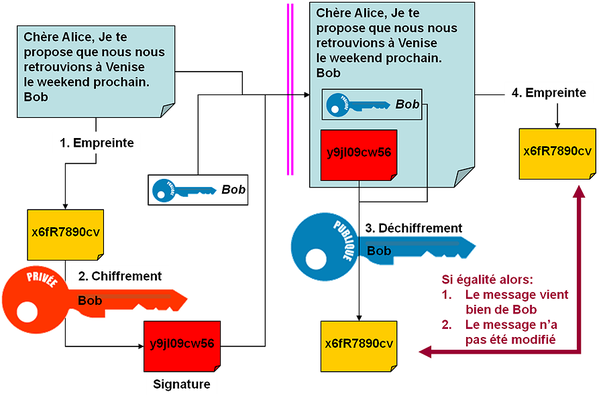
\includegraphics[scale=1.025]{signature_num.png} 
\caption{Signature numérique} 
\end{figure} 


\end{document}
